%
% Sample SBC book chapter
%
% This is a public-domain file.
%
% Charset: ISO8859-1 (latin-1) áéíóúç
%
\documentclass{SBCbookchapter}
\usepackage[utf8]{inputenc}
\usepackage[T1]{fontenc}
\usepackage[brazil,english]{babel}
\usepackage{graphicx}
\usepackage{array}

\setcounter{chapter}{4}

\author{Sam Haynes}
\title{{Limitations} of composability of cis-regulatory elements in messenger RNA}

\begin{document}
\maketitle

\begin{abstract}
This chapter is about finding short cis-regulatory motifs in the 3'UTR of mRNA transcripts and detecting if their regulatory behaviour is dependent on the context of the whole transcript. This could be the context of the 5'UTR, ORF or the 3'UTR. We also introduced two motifs at the same time to see if they interact with each other. To begin, a literature search found 69 motifs previously identified as being enriched in transcripts that bind proteins or are highly expressed. Then, a linear model predicting transcript half life using codon usage, 3'UTR length and the presence or absence of these motifs was trained on two independent half life data sets. Using a greedy algorithm that maximised the AIC of the model, the 69 motifs were shortlisted to just 4 likely contributors. These 4 chosen motifs were inserted into two different native terminators and removed from one terminator that they appear in natively. Each motif-terminator set was also pair with three different promoters creating a library of 20 constructs. Using qPCR to detect changes in the expression of these constructs we then determined whether these motifs have the same effect in different contexts or whether they contribute the same across transcripts. We confirmed these effects are repeated in protein expression and in RNA-Seq expression. Finally we attempted to see if these transcripts had different PolyA sites in the total and decay populations but found different in only one case.
\end{abstract}

\section{Chapter 4 Introduction}

Predicting expression of construct reliably is crucial for the progress of synthetic biology.

Understanding gene regulation pathways requires more nuanced approaches that enable non-linear interactions. 

Deep learning algorithms remain black-boxes that can learn complex behaviour but not in an interperatable way.

Typically since the creation of modular synthesis tool kits the importance of considering context specific effects when combining parts is either ignored or considered not worth while.

 First we provide further evidence for the important of considering interactions between regulartory regions by creating chimera constructs of promoter-ORF-terminator combinations.
 
\section{Chapter 4 Results}

\subsection{Chimera project}

The mRNA abundance and protein abundance of these constructs we quantified using qPCR and plate reader measurements.

qPCR was determined relative to the PKG1 constructs using tidyqpcr.

The platereader measurements were determined using the omniplate python package which uses a Gaussian Processes algorithm to find the fluorescence at max growth rate.

We showed that the contribution from promoter choice is the largest, then the contribution from terminator choice but there was also unpredictable differences in a terminators contribution to gene expression depending on ORF and promoter.

\subsection{RNA-binding motifs}

We then considered whether this context dependence is repeated by cis-regulatory elements within the promoter/orf regions.

Using a literature search we found 69 suspected regulatory motifs found in the 3'UTrs of transcripts.

To reduce the list of 69 putative RNA binding protein motifs to a shortlist of 4, we trained a linear model to predict half life using the presence or absence of these motifs. Although many of the motifs did not have a recognised regulatory protein or pathway associated with them, the few that did were associated with mRNA degradation proteins such as PUF4. Therefore, we decided shortlisting the motifs according to through that best predict RNA half lives would be a feasible way of enriching for functional motifs that we could then inspect for context dependence. As all the motifs of interest were found predominately in the 3'UTRs of mRNA transcripts we used an extended yeast genome annotation, which includes the longest 3'UTR isoforms, to find the appearance of motifs in a gene. We found two genome-wide, non-invasive half life data sets available to train the model on. The data sets measure half life by introducing an alternative uracil nucleotide for a limited time (30 minutes) and measure the change in counts of transcripts created with this nucleotide as a measure of decay. The two data sets correlated reasonable well Figure 1A but the Cheng et al data set used multiple time points to infer decay rates and therefore was more sensitive to shorter half lives. We also found a previous study that predict motif contributions to gene expression which also modelled two other key predictors of half life: codon usage and length. We deciding to introduce these predictors to reduce the likelihood of confounding effects. We trained the model on both decay datasets and saw that we predicted a reasonable amount of the variation in transcript half life from this alone.To shortlist the motifs, we used a greedy algorithm maximising the AIC. This a penalised likelihood model that balances model complexity (i.e. the maximum number of motifs that the model can use at the same time) with accuracy. We then selected motifs that were significant in both data sets and had predicted contributions with reasonably high magnitudes. We also checked that these motifs occur frequently in native terminators. It is also clear that, as previous studies have suggested, it is difficult to detect motifs that increase half life. Therefore, we chose one motif suspected to increase half life but only occurs occasionally. The contributions to gene expression for each shortlisted motif correlated well for all but one motif.

\begin{figure}[p]

{\centering 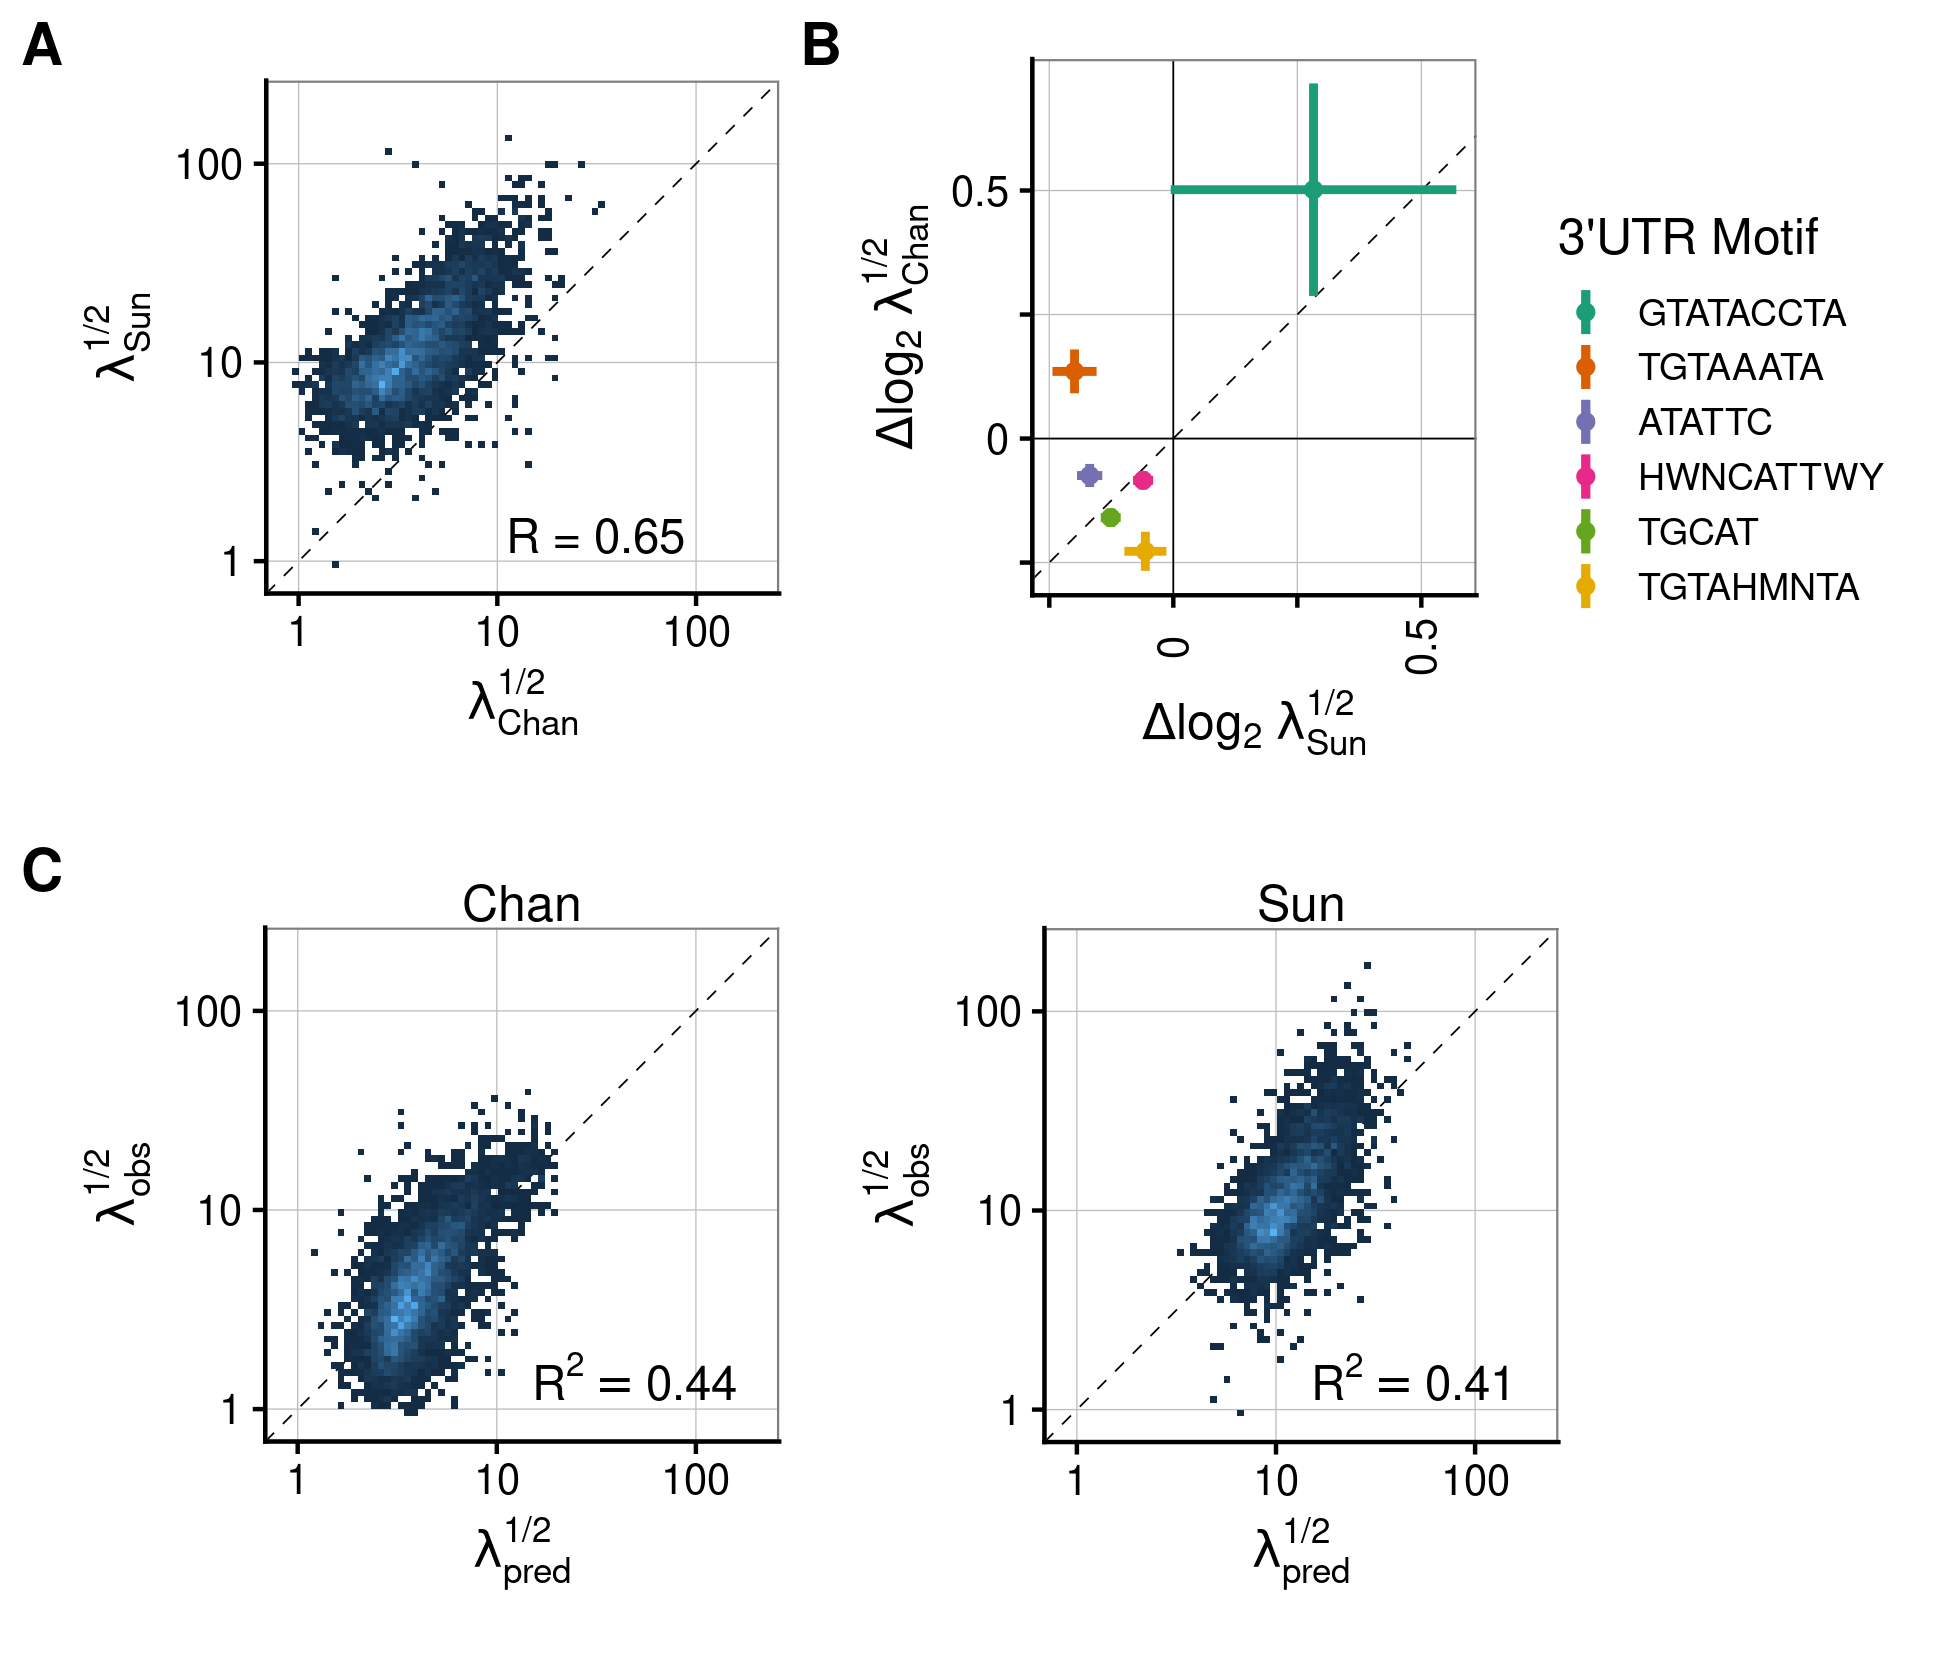
\includegraphics[width=0.98\linewidth]{figures/hlife_model_multi_fig} 

}

\caption{\textbf{A linear model of transcript half-life quantifies the effect of candidate terminator motifs on half-life.} (\textbf{A}) Correlation between the 2 transcript half-lives (\(\lambda\)), in minutes, reported in the (38) and (46) datasets. (\textbf{B}) Predicted contributions to log2 half-life for chosen motifs in the (38) and (46) datasets. (\textbf{C}) Predicted vs actual transcript half-lives calculated by a linear model of codon and motif usage trained on the (38) and (46) datasets.}\label{fig:hlife-decay-model}
\end{figure}


We had to make amendments for the fact that these motifs were conservation sequence and not actually unique in every case.


Two native terminators were chosen as hosts for the cis-regulatory motifs of interested: TSA1 and RPS3. They were selected for having no motifs of interest in them natively, short 3'UTR lengths and high expression. Three 9bp motif insertion sites were created, extending the native 3'UTR by 27 bp. The exact position of these insertion sites were dictated by the position the motifs of interest appear in natively, avoiding host terminator secondary structures, leaving efficiency and position elements required for cleavage and poly adenylation and ensuring the motifs appear within the major poly(A) isoform. Motifs with lower magnitude contributions were inserted in duplicates, with the insertion site left with a random sequence. One construct has all three insertion sites occupied as it contained two different motifs to check for interaction effects. As a control we also created a control terminator with random sequences at all insertion sites. Figure 1A shows the positions of the three insertion sites for both terminators and which motifs were inserted where. The terminator constructs were paired with three different promoters: the native promoter for the host terminator, a high expression PGK1 promoter and a low expressing SRO9 promoter.

The mRNA abundance of each construct was measure using qPCR. The delta delta Cq was calculated relative to the control construct of each set of promoter-terminator constructs. Figure 1B shows that the all of the motifs with predicting effects reducing transcript half-life correlate with a decrease in transcript abundance in RPS3 transcripts. The same is true for TSA1 transcripts show in Figure 1C. However, the one stabilising motif does not have a consistent effect on gene expression across the transcripts. It is also important to note that there isnt a large difference in expression between the WT constructs and the control constructs with random sequences inserted.  

\begin{figure}[p]

{\centering 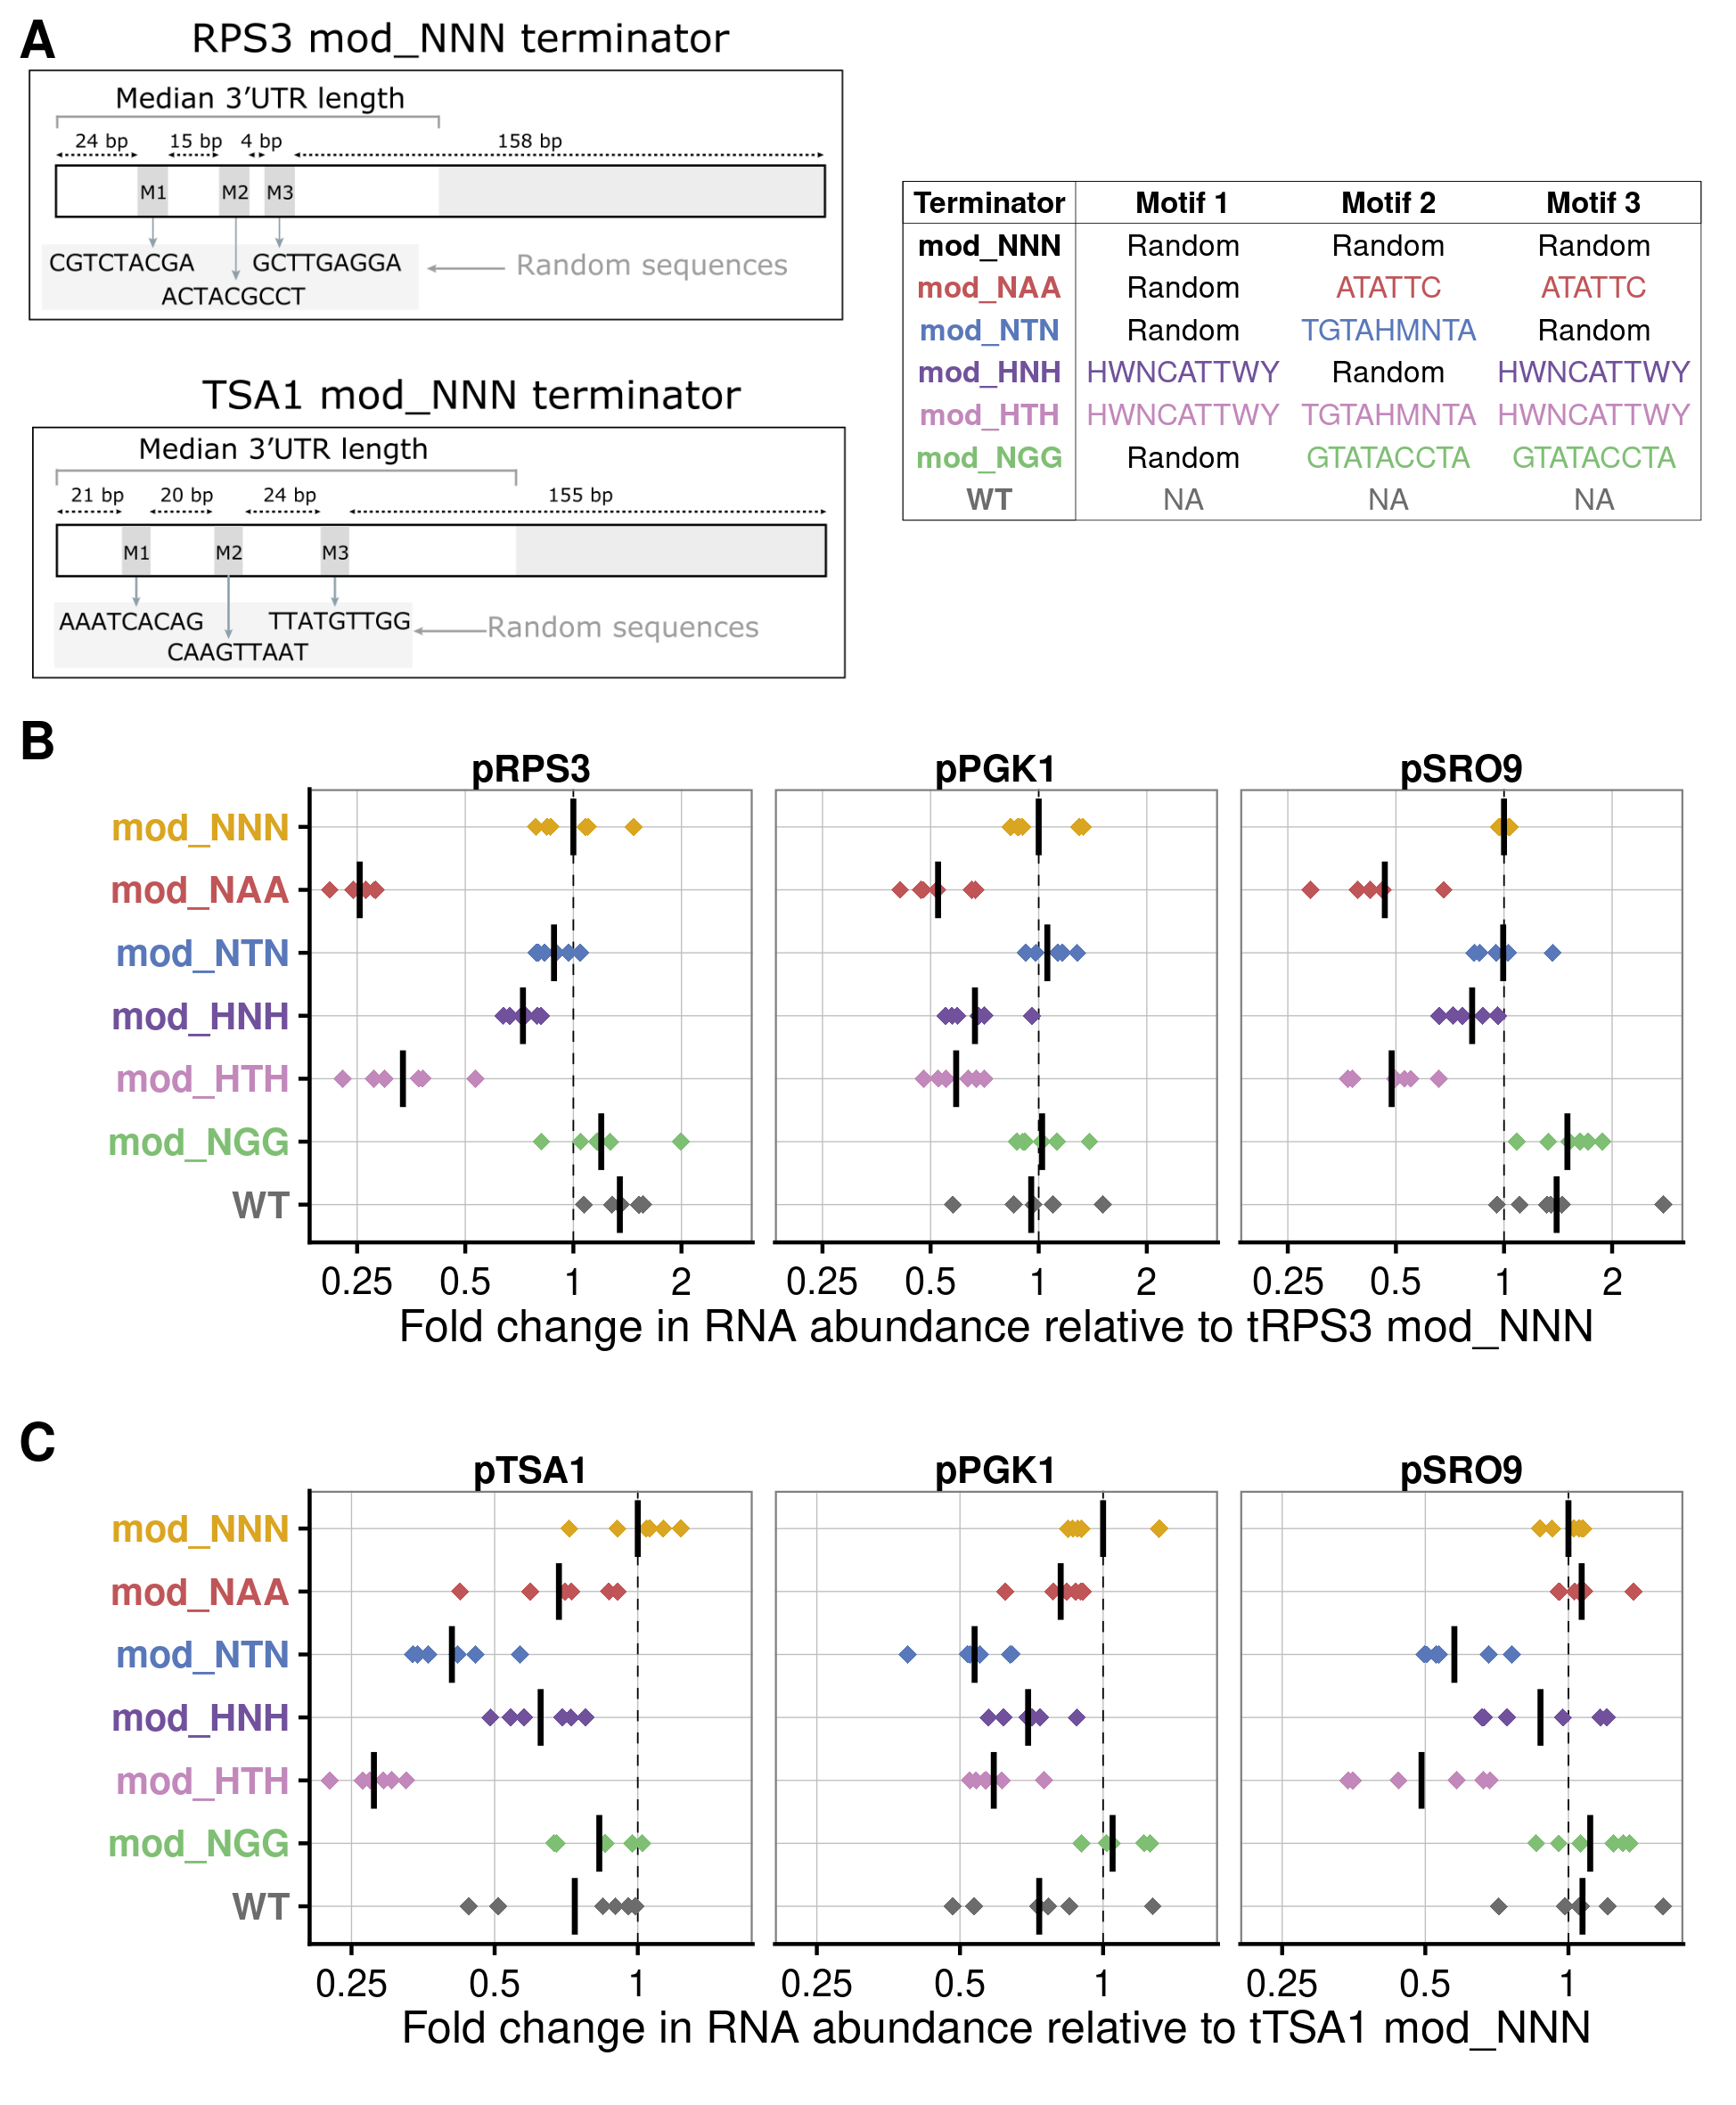
\includegraphics[width=0.98\linewidth]{figures/insertion_constructs_design_and_qpcr} 

}

\caption{\textbf{Motifs inserted into RPS3 and TSA1 host terminators change transcript abundance in RT-qPCR measurements.} (\textbf{A}) Design of motif insertion sites in native RPS3 and TSA1 terminators, highlighting random insertion used as a negative control. (\textbf{B}) Fold changes in transcript abundance for tRPS3 constructs paired with 3 promoters: pRPS3, pPGK1 and pSRO9. (\textbf{C}) Fold changes in transcript abundance for tTSA1 constructs paired with three promoters: pTSA1, pPGK1 and pSRO9. Each diamond represents a biological replicate, averaged over 3 technical replicates. The vertical line represents the mean of all 6 biological replicates. Fold changes are relative to the abundance of the mod\_NNN construct, i.e. $2^{\Delta\Delta Cq}$ (see methods).}\label{fig:tRPS3-tTSA1-design-and-qpcr}
\end{figure}

A third native terminator was selected which contained three of the four motifs in its 3'UTR. PIR1 contains an ATATTC, an TGTAHMNTA, and three HWNCATTWY motifs. The exact sequence of the three HWNCATTWY motifs differ from each other and from the sequence inserted into the other two terminators. Figure 1A shows the position of these motifs in the 3'UTR PIR1 and the table in Figure 1B shows the combination of constructs created to explore the behaviour of these motifs. To remove these motifs from the native sequence we replaced the motif with a random sequence of the same size. We also check that these randomly generated sequences do not unintentionally introduce any known motifs.First we created three constructs each with all copies of one motif removed. We also created constructs with only one of the different versions of HWNCATTWY removed to explored the positional and sequences effects. Finally we created constructs with the HWNCATTWY motifs and one of the other two motifs removes to check for interaction effects. The qPCR abundance was measure realtive to the WT terminator as no control construct was needs to check for changes in poly(A) length. The qPCR results show that the removal of any of the the suspected decay motifs leads to an increase of transcript abundance. Also, as more motifs were removed the greater the increase in transcript abundance. Similar patterns in transcript abundance were seen across the three promoter pairings. 

\begin{figure}[p]

{\centering 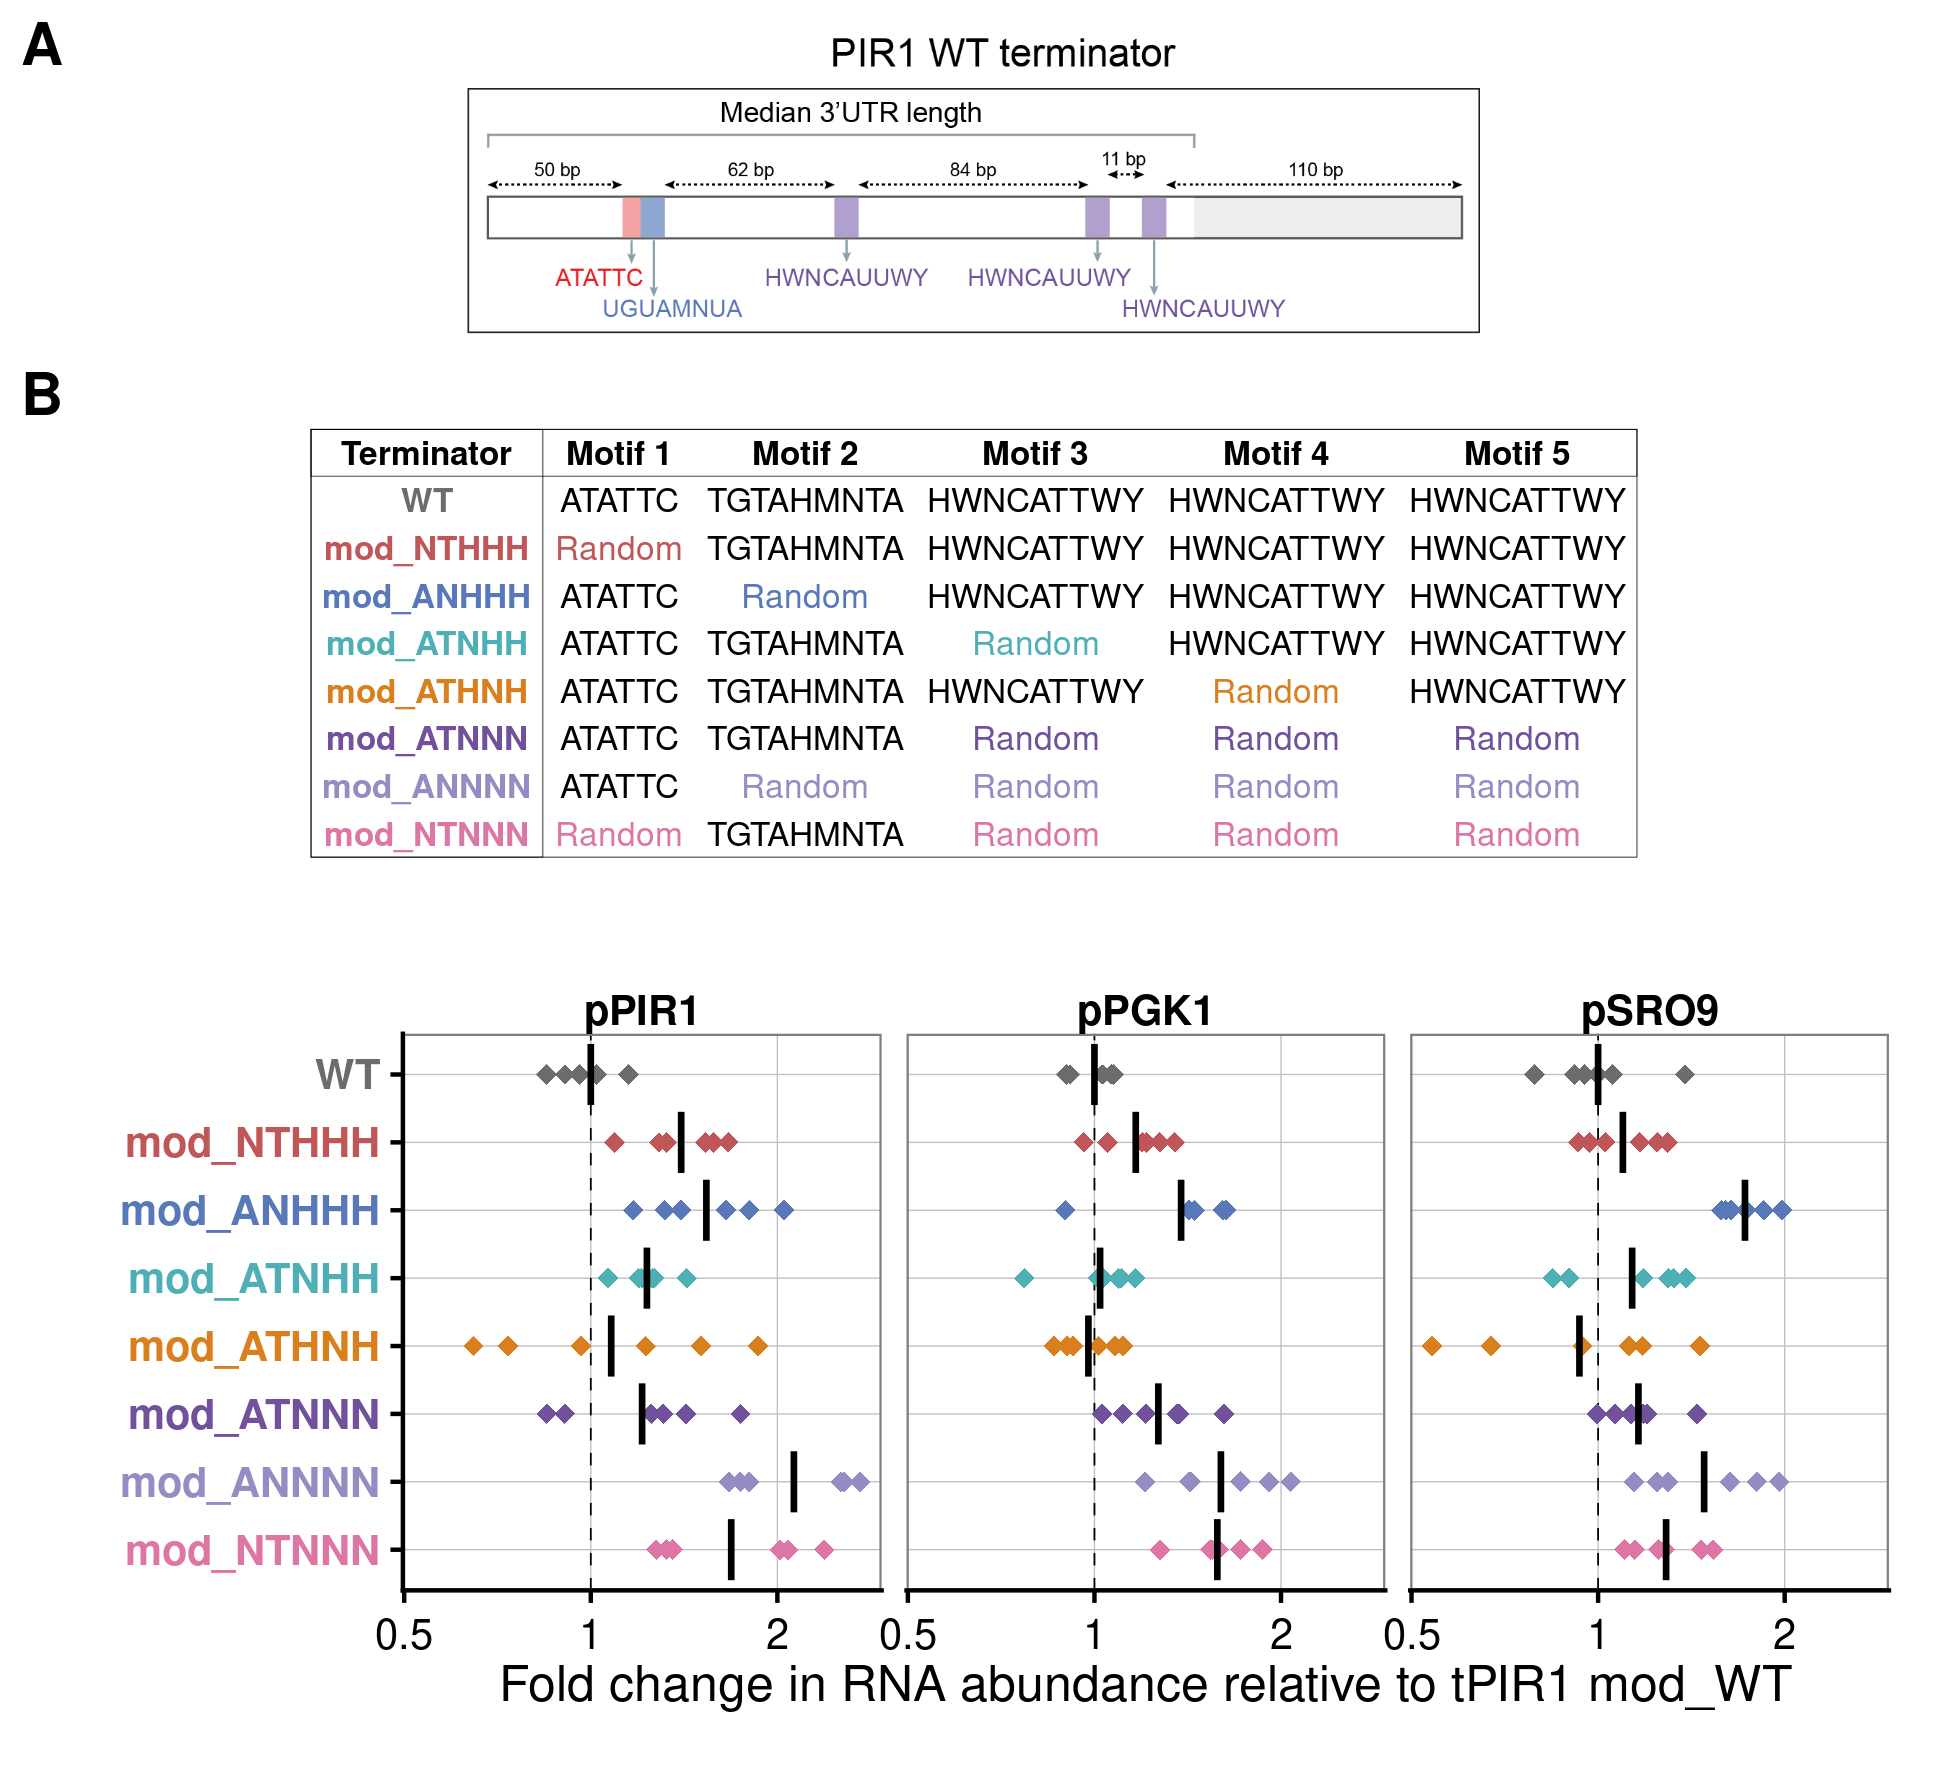
\includegraphics[width=0.98\linewidth]{figures/tPIR1_design_and_qpcr} 

}

\caption{\textbf{Motifs removed from PIR1 host terminators change transcript abundance in RT-qPCR measurements.} (\textbf{A}) Design of PIR1 constructs with combinations of motifs replaced by random nucleotide sequences. (\textbf{B}) Fold changes in transcript abundance for tPIR1 constructs paired with 3 promoters: pPIR1, pPGK1 and pSRO9. Each diamond represents a biological replicate, averaged over 3 technical replicates. The vertical line represents the mean of all 6 biological replicates. Fold changes are relative to the abundance of the WT construct, i.e. $2^{\Delta\Delta Cq}$ (see methods).}\label{fig:tPIR1-design-and-qpcr}
\end{figure}

Finally we also looked into whether two motifs inserted together have the same effect no matter what or if they interfered/cooperated with each other.

Again investigated the construct mRNA abundance with qPCR but relative to the control construct with randomly generated sequence in the insertion sites.

We found mRNA abundance correlates well with protein florescence using a subset of constructs.

\subsection{Poly(A) site usage}

We wanted to confirm that our motif insertion also did not change the polyA sites used, as this can significantly effect abundance.

We do QuantSeq Rev which has a polyA anchored reads to determine polyA isomers and found a difference in one case.

This RNA-Seq results also correlated with qPCR data.

Also, we used 5PSeq to determine polyA usages in transcripts flag for decay with 5' cap removed but they didn't show any significant difference from the QuantSeq.

\section{Chapter 4 Conclusions}

Motifs can be context dependent for a whole host of reasons.

They may have multi-faceted uses: binding certain proteins inside the nucleous and in the cytoplasm or during a heat shock response compared to normal exponential growth phases.

They may be chaperon proteins for the actual effector protein which may only bind/phosphrelate ect in certain locations in the cell.

ASH1 for example only suppresses translation of its target transcripts in the mother cell. Once it reaches the bud cell it is phosphorylated and stops being able to bind to its target and so the motif becomes useless.

Motifs may also require presentation in certain secondary structures be successfully bound by their targets.

Alternatively, motifs may need to be repeat or appear with the other motifs to fully complete their objective.

Introducting non-linear models that can account for complex interactions between secondary structure, transcript location and motif interactions can help develop interperatiable models that better predict construct expression.

Random forestion/partition regression models are quick, easier to conceptialise and highly developed non-linear models that have been used in other work previously.

\bibliographystyle{apalike}
\bibliography{sbc-template}

\end{document}